\section{Introduction}
\label{sec:intro}

Pretrained Language Models (PLMs) are used in a wide variety of NLP tasks and applications. These are large neural networks that operate under a pretrain-finetune paradigm: first, models are \emph{pretrained} over a large text corpus, and then \emph{finetuned} on a downstream task of interest. PLMs are typically thought of as good representation learners, supplying some basic language understanding capabilities that can be used with ease on many downstream tasks.

A desirable property from a good language understanding component is consistency. That is, the ability to make consistent decisions, reflecting a systematic generalization ability to understand language, regardless of language variability. %\sr{This sense of ``consistency" focuses on the ability to reason in a way that is invariant to meaning-preserving alternations. Note this differs from the way we initially thought about consistency: a model that always predicts the same answer is also ``consistent" but surely doesn't express this meaning of consistency. It's ok to focus on the meaning we focus on here, but if we do so, shouldn't we focus in the experiments on cases where the model initially predicted correctly? our current evaluation doesn't align, to my understanding, with this definition in the intro.}.  \ar{The definition of inconsistency in my mind, is having beliefs that result in a contradictions. The paraphrase thing is one way to test this for some applicable relations (if you believe 'X was born in Paris' and 'The birthplace of X is Delhi', this results in a contradiction). We can make this clearer.} 
For example, predicting the same answer in reading comprehension tasks, regardless of paraphrases \cite{consistent-qa}, consistency inferences in coreference resolution \cite{denis2009global,chang2011inference} or making summaries factually consistent with respect to the original document \cite{kryscinski2020evaluating}.
This property is important for many tasks involving language and is hard to obtain solely in a supervised setting. 
% Ideally, a PLM such as BERT or RoBERTa \cite{bert,roberta} would arrive with such capability, persist during the finetuning step and allow the new model to make consistent predictions. 
Ideally, a PLM such as BERT or RoBERTa \cite{bert,roberta} would learn such capability during the pretraining phase and then transfer it to the down-stream task. %\ar{I think we can be more explicit here of how consistency can act as evidence of a more general and systematic ability to understand language.}


\begin{figure}[t!]
\centering

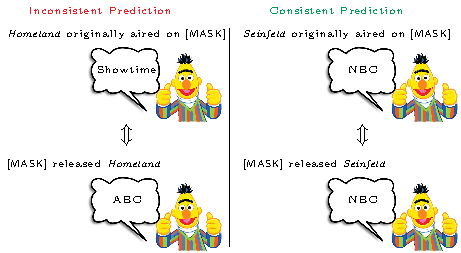
\includegraphics[width=1.\columnwidth]{figures/overview}

\caption{Overview of our approach. We begin with KB triplets (\textit{subject}, \textit{object}, \textit{pattern}), of which we feed the (\textit{subject}, \textit{[MASK]}, \textit{pattern}) into a PLM. 
We expect that a consistent model would predict the same answer for every two tuples of $(subject, pattern_1)$, $(subject, pattern_2)$ with an entailment connection between them.}
\label{fig:overview}
% \vspace{-6mm}
\end{figure}


Recently, with the rise of PLMs, the question of whether these models can be used as KBs has been raised and gained popularity \cite{lama,petroni2020how,alpaqa}. However, an important property of KBs, especially in automatically constructed KBs, is consistency.
One of the biggest advantages of using a PLM as a KB is the ability to query it in natural language and to not rely on a specific schema.
Thus, expecting that the PLMs would abstract away the language, and map queries in natural language into a meaningful representation, queries with identical meaning should yield the same answer, even if their language differs.
For example, ``\textit{Homeland} was released on [MASK]'' should produce the same answer as ``\textit{Homeland} was originally aired on [MASK]''.
Studying inconsistencies of LM-KBs as a testbed can also teach us about the organization of `knowledge' in the model, or lack thereof. Failure to do so may also point to other issues in representations, such as the similarity between antonyms and synonyms \cite{nguyen2016integrating}.

In this work, we study consistency from the factual knowledge perspective, that is, the ability to extract factual information while staying invariant to paraphrases.
Our setup relies on zero-shot evaluation, which allows us to
inspect these capabilities in models directly, without
adding biases that arise from finetuning on a specific
dataset. This allows us to understand if consistency was learned during pretraining, and will allow to track and improve this property in future work. %\sr{Question: how do we separate between lack of consistency due to the extraction method (maybe other extraction method would yield more consistent predictions), and an inherent lack of consistency in the model's behavior?}


We propose a new benchmark that measures consistency in PLMs, using factual knowledge that was claimed to be partially encoded in them (\S \ref{sec:framework}).
This benchmark, \resource{}, is a manually curated resource
that provides patterns -- short textual prompts -- that are paraphrases of one another, with @@ paraphrases describing 40 relations, such as \textit{born-in}, \textit{works-for} (\S \ref{sec:rel-graph}).
Then, expecting from a consistent model to predict the same answer for all the patterns, we test multiple PLMs for consistency over knowledge.
An overview of the probe is displayed in Figure \ref{fig:overview}.
Using \resource{}, we are able to probe for consistency in PLMs (\S \ref{sec:setup}), including BERT, RoBERTa and ALBERT.
We find that overall, current models perform poorly on the consistency benchmark, although there is a high variance between the different relations (\S \ref{sec:experiments}). 

Finally, we propose a method that improves the consistency capabilities of models, with an additional consistency loss (\S \ref{sec:adding_consistency}). Our experiments show promising results and achieve better consistency performance on new relations, but there's still a big gap before achieving consistent models.
% Extending upon previous work that showed that factual knowledge can be extracted to some degree \cite{lama,alpaqa}, we extend their proposed patterns that were used to extract that information, and manually write paraphrases to the original patterns.


% \resource{} contains 40 relations from the T-REx dataset \cite{trex} provided by LAMA \cite{lama}, such as: \textit{born-in}, \textit{is-a-citizen}, \textit{works-for}, etc (\S \ref{sec:rel-graph}).
% The paraphrases were built by experts, and provide a high-quality resource.
% \nk{jump from one graph to multiple graphs} 
% Each of these graphs contains between @@-@@ different nodes, where each node is a pattern, e.g. ``[X] was aired on [Y]'', where \textit{[X]} and \textit{[Y]} are slot fillers for a subject and object.
% Moreover, each edge is also annotated with the modification type (e.g. syntactic, lexical) \sr{I am not sure we need to mention these in the intro, given the pretty narrow / heuristic way we define those}.
% Examples of edges of the graphs are displayed in Figure \ref{fig:graph}.


%%%%%%%%%%%%%%%


% By combining the \resource{} with the proposed framework, we are able to test different PLMs and how strong their consistency capabilities are.
